\documentclass[format=acmsmall, review=false]{acmart}

\usepackage{acm-ec-18}

\usepackage{booktabs} % For formal tables

\usepackage[ruled]{algorithm2e} % For algorithms


\renewcommand{\algorithmcfname}{ALGORITHM}
\SetAlFnt{\small}
\SetAlCapFnt{\small}
\SetAlCapNameFnt{\small}
\SetAlCapHSkip{0pt}
\IncMargin{-\parindent}
\newcommand\mycommfont[1]{\footnotesize\upshape\textcolor{blue}{#1}}
\SetCommentSty{mycommfont}

\begin{document}
% Title portion. Note the short title for running heads 
\title[New strategies for improving kidney exchange]{New strategies for improving kidney exchange}  
\author{Submission 42}

% note that the abstract must come before \maketitle
\begin{abstract}
[[Kidney exchange is great, provides a way to increase number of lives saved]] [[Most algorithms static, don't think about future]] [[There might be ways to improve, but literature still small]] [[This work adds two contributions to the literature]] [[Direct prediction method, MAB-based methods]] [[The latter can improve the average number of kidneys exchange by 3\% over the myopic algorithm]]
\end{abstract}

% note: this command has been disabled to remove the ACM copyright block. Sorry...
%\thanks{This work is supported by the National Science Foundation,
%  under grant CNS-0435060, grant CCR-0325197 and grant EN-CS-0329609.}


\maketitle

\section{Introduction}

[[Kidney exchange]]

[[Will interchangeably use the words 'node', 'vertex' and 'pair']]

\paragraph{\textbf{Main idea}} We propose and compare two new approaches to improve the number of matching in kidney exchange, namely the \emph{direction estimation} method and the \emph{multi-armed-bandit} method. The former recasts the dynamic kidney exchange problem as a binary classification task: for each pair in the pool, we should predict a 0-1 label representing whether they should be matched today, or left for the future. The latter chooses exchanges that are less likely to produce ``regret" in the future (under a specific definition of regret that we elaborate on later).

Each approach faces different challenges. In the \emph{direct estimation} approach, one challenge is that an important part of our data -- the compatibility graph -- lives in a non-Euclidean space, and it is not obvious how to use it as an input to a classification algorithm. We attempt to apply a variety of new methods from the graphical signal processing literature to tackle this problem. An additional challenge is that traditional classification algorithms are not equipped to produce dependent labels, but in our setting whether or not we decide that a certain pair is to be matched today ought to be related to our decisions about everyone else in the pool. To overcome this we use recurrent neural networks and draw from the [[[[]]]]

In the \emph{multi-armed bandit} method, the main issue is that the enormous branching factor of our problem precludes an accurate estimation of regret for each possible exchange. Here, we develop a novel algorithm that iteratively chooses to match one additional pair or decides


\paragraph{\textbf{Main results}} We conduct simulations following three models from the kidney exchange literature, which we call \emph{environments}. The three environments differ by their rules regarding blood- and tissue-type compatibility.

We apply our methods to each of these environments and compare them to a myopic algorithm (representing how kidney exchanges are currently conducted), and to infeasible optimal algorithm. Comparison is made in terms of average number of pairs matched per period, and the average is taken over a long period of time (i.e., much longer a node's mean sojourn).

In all environments, we observe that the \emph{direct estimation} unfortunately does equally well or worse than the myopic algorithm. However, the \emph{multi-armed bandit} method is able to improve upon it by 0.5-5\% in terms of the number of average pairs matched per period. Moreover, we observe that there is still a moderately large performance gap between our algorithms and the infeasible optimal.


\subsection{Related literature} This paper pulls ideas from microeconomics and matching theory, and uses methods drawn from computer science, machine learning, and operations research. Let us take a brief look at these fields in turn. 

\paragraph{Dynamic kidney exchange}

\paragraph{Computer science}



%%%%%%%%%
\section{Simulation environments}

\paragraph{Notation} 

\subsection{Common features across environments}

\paragraph{Poisson entry, Geometric death} At time point, the number of new incoming pairs is drawn from the $Poisson(r)$ distribution, where $r \in \mathbb{N}$ denotes the \emph{entry rate}, and equals the expected number of entrants per period. Upon entrance, each pair independently draws the length of their sojourn from the $Geometric(d)$ distribution. The parameter $d \in \mathbb{R}$ is the \emph{death rate}, and its reciprocal $\frac{1}{d}$ is the expected sojourn length. We note that, due to the memoryless property\footnote{If $X \sim Geometric(p)$, then $P(X > t+s | X > s) = P(X > t)$} of the Geometric distribution, the amount of time a pair has waited in the pool gives us no information about how much time they have until their death.

\paragraph{Minimum set of observable characteristics} In every environment, at least two characteristics are relevant and observable: the major blood type groups (A, B, O or AB) of the patient and donors, and how long the pair has been in the pool. On the other hand, death times are never observed.

\paragraph{Binary preferences} In this work we abstract from these concerns and consider every exchange to be equally desirable, so long as it is available. This is the same assumption as used in \cite{roth2005pairwise}, 

\subsection{ABO Environment}

In the \emph{ABO environment}, a pair's observable characteristics are their current waiting time and dummies representing ABO blood types of its patient and donor. Compatibility between two distinct pairs is based only on blood-type compatibility. Blood types are drawn independently for patient and donor from the US population (roughly O:48\%, A:36\%, B:11\%, AB:4\%). In addition, we make an assumption previously used in \citet{unver2010dynamic} and allow for incompatibility between a donor and their own patient. The reason for this additional assumption is that, if there were truly no tissue type compatibilities, we would never observe pairs of type (AB,$\cdot$), ($\cdot$, O), or (A,A), (O,O), (B,B), and (AB,AB), since their donors would be automatically compatible with their patients and they would never participate in an exchange. Following \citet{zenios2001primum}, we assume that for such patients the probability that a donor and their patient are incompatible is $p_c = 0.11$. Arrival rates are adjusted accordingly, e.g., the arrival rate of $(A,O)$ pair is proportional to $0.48 \times 0.36 \times 0.11 \approx 0.019$.

\subsection{RSU Environment}

The \emph{RSU} environment drawn from the setup in \cite{roth2007efficient}. Observable covariates are dummies representing patient and donor ABO blood types, current waiting time, and a \emph{calculated panel reactive antibody (cPRA)} level that governs the probability of a crossmatch with a random donor.\footnote{The original \cite{roth2007efficient} paper called this simply \emph{PRA}. In real life there is an important distinction between the two measures, but for the purposes of a simulation model this distinction is immaterial. We keep the name \emph{cPRA} for consistency with OPTN environment.} The lower the cPRA, the higher the number of potentially compatible pairs.

The simulation process is as follows. First, we draw a pair in the same manner as in the ABO environment. Next, we draw if the patient is a female (with probability around 41\%), and if so we also draw whether her donor is her husband (spouses comprise about 49\% of donors). Finally, we draw a  cPRA level for the patient (Low: 70.1\%, Medium: 20\%, High: 9.9\%). This cPRA level determines the probability that they can receive a kidney from any donor, including their own: patients with low cPRA have a 5\% probability of positive crossmatch with a random donor; patients with medium cPRA have a 45\% chance, and patients with high cPRA have a 90\% chance of a crossmatch. If a patient is bloody or tissue-type incompatible with their own donor, they enter the pool. In addition, if the patient is female and her husband is the donor, the probability of positive crossmatch for low, medium and high cPRA patients goes up to 28.75\%, 58.75\% and 92.25\%. This last adjustment reflects the fact that women tend to produce antibodies against their husbands' antigens during pregnancy.

Once in the pool, the pair immediately forms directed edges with the existing pairs, again following the patient cPRA distribution. The resulting random graph is akin to a Erd\"{o}s-R\'{e}nyi $G(n,p)$ random graph where the probability of forming edges is heterogeneous across different pair types.

\subsection{OPTN Environment}

In the \emph{OPTN environment}, we use historical data collected by the United Network for Organ Sharing (UNOS) data provided in the Standard Research and Analysis (STAR) dataset. The STAR dataset contains information from all patients that were ever registered to the kidney waiting list in the United States for the past three decades, as well as from living donors that participated in an transplant. From this original dataset, we excluded patients that were registered for more than one organ (including kidney+pancreas), patients that were not waiting for their first kidney transplant, and patients and donors with incomplete HLA profile information. The resulting historical dataset still contained 117813 patients and 9337 living donors.

\paragraph{Patient and donor cPRA} We added two additional variables to the original dataset: a \emph{patient cPRA} and a \emph{donor cPRA}. While the patient cPRA is a measure of patient tissue-type incompatibility with a random donor \cite{cecka2010calculated}, our \meph{donor cPRA} is a novel measure of the opposite direction -- how frequently a donor is tissue-type incompatible with a random patient.\footnote{We thank Itai Ashlagi for the suggestion of a donor cPRA.} Both were computed empirically: for each patient our dataset, we checked the how many donors exhibited antigens that are unacceptable for the patient in any of the A, B, Bw, C, DR, DPB, DQ, and DQA loci, and assigned this positive crossmatch probability as their patient cPRA; for the donors, we worked in the opposite direction by calculating the frequency of patients who exhibited antibodies against their donor's antigens, and that became their donor cPRA. Figure \ref{fig:cpra} shows the distribution across the entire population.\footnote{We should remark that we found a very different patient cPRA distribution than the one in the OPTN dataset. This may have been because: in real life cPRA is computed using deceased donor data, whereas we use living donor data; we have used different HLA equivalence tables; OPTN uses a more sophisticated model based on population genetics.\cite{optn2013cpra}}


\begin{figure}
\centering
\includegraphics[width=\textwidth]{/Users/vitorhadad/Documents/kidney/matching/phd_thesis/figures/computed_cPRA.pdf}
\caption{Patient and donor cPRA computed from historical data.}
\label{fig:cpra}
\end{figure}


\paragraph{Artificial dataset} Next, we created an artificial dataset by randomly drawing patients and living donors from the historical dataset and checking for blood-type compatibility, and tissue-type compatibility as explained above. Compatible pairs were discarded. We iterated in this manner to construct a dataset of about one million incompatible pairs. Its columns are a set of dummies representing patient and donor blood times, a set of dummies for each allele in each HLA locus, and 

At every simulation period, a random number of pairs are drawn from this dataset.

[[[[Algorhtm can still see original alleles. Patient and donor cPRA offer "long-run" measure of compatibility]]]]


%%%%%%%%
\section{Methods}

\subsection{Objective and benchmarks}

In this work, we focus on maximizing the average number of matched pairs over $T$ periods, where $T$ is a large number relative to the rates of patient entry and death. We are interested in how our new methods perform relative to the following two benchmarks.

\paragraph{\textsc{Myopic}}

This algorithm finds the maximal matchings at every period, and clears it immediately. It disregards all observable characteristics of each pair, and in particular it disregards that some pairs might be useful to keep certain pairs may be easier or harder to match. In doing so, it may forgo the opportunity of matching a hard-to-match patient today, or postpone an easy-to-match pair for later. In essence, this is an approximation to what kidney exchanges currently do.

\paragraph{Optimal (\textsc{OPT})} This infeasible algorithm (henceforth OPT) does away with the uncertainty arising from the temporal structure of the problem: it knows exactly which pairs will come into the pool, as well as their arrival, and the duration of their sojourns. This algorithm is essentially a large static kidney matching problem, except that the set of available exchanges has the additional constraint that a cycle cannot exist between two vertices if their sojourns fail to overlap.

\textbf{Remark} \textit{How much is there to be improved upon?} [[]]

\begin{figure}[H]
\centering
\hspace*{-3.5cm}
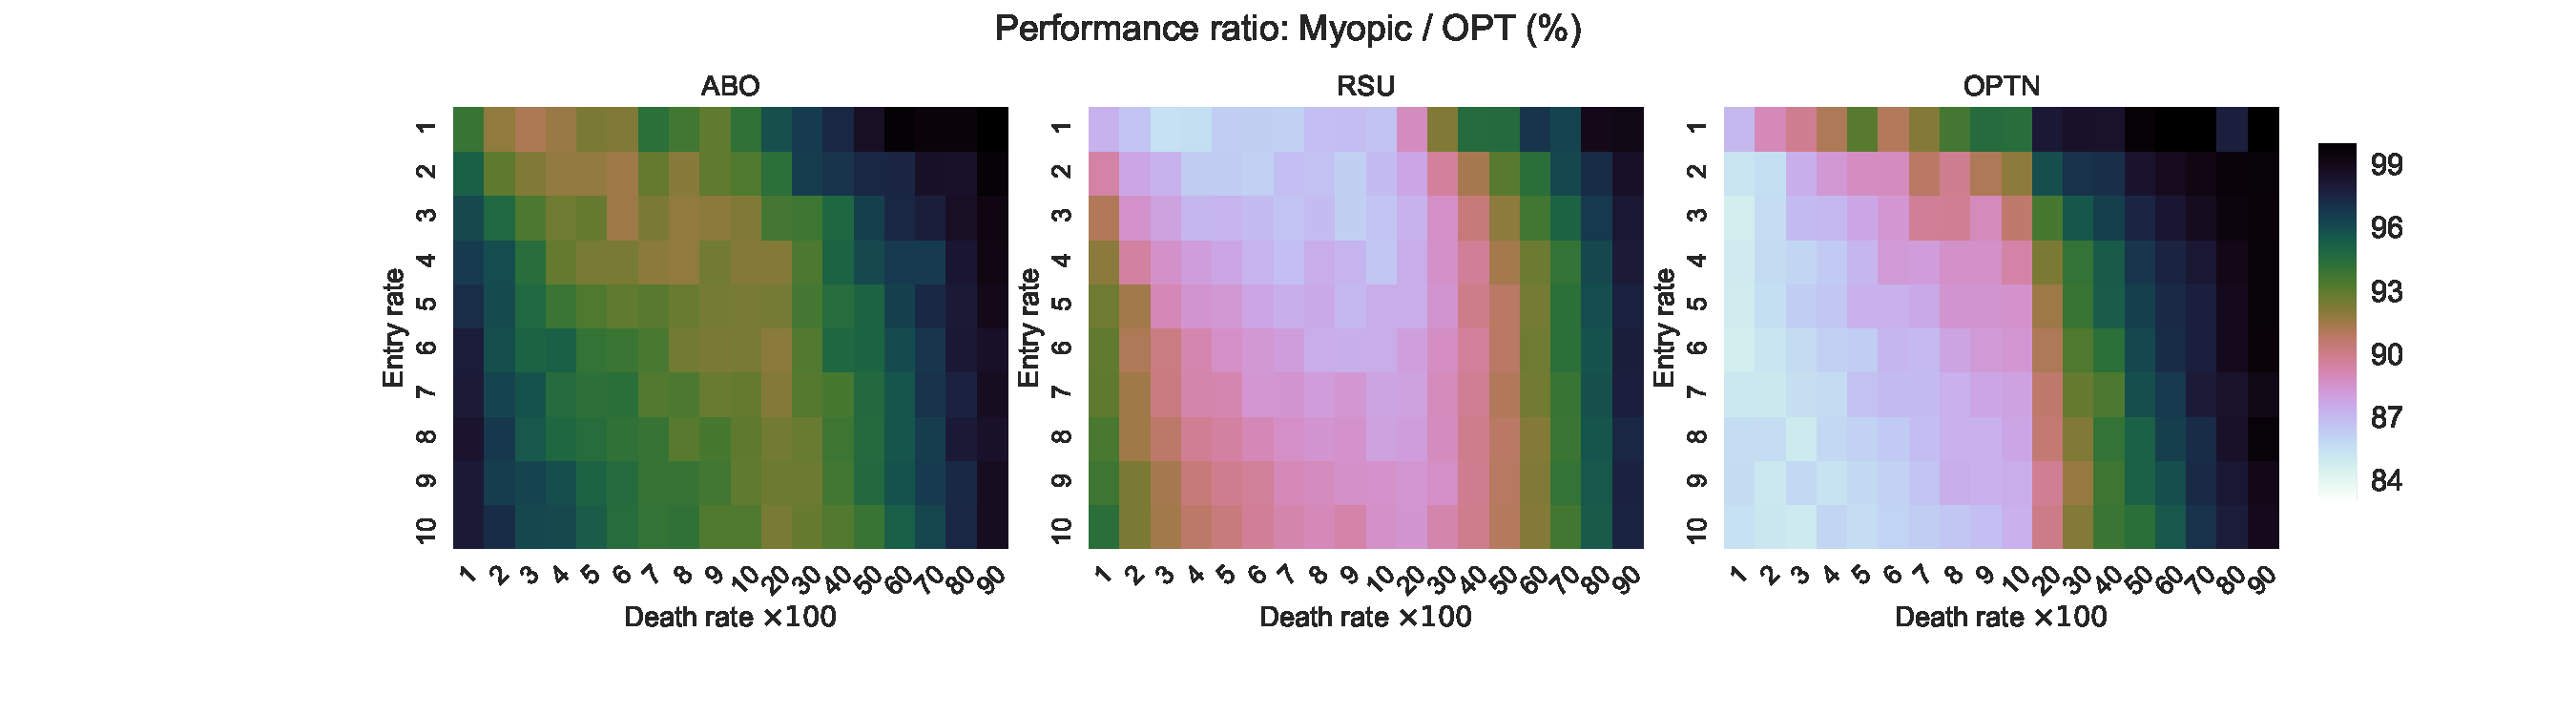
\includegraphics[width=1.4\textwidth]{/Users/vitorhadad/Documents/kidney/matching/phd_thesis/figures/greedy_opt_comparison_mcl2_2.pdf}
\caption{Ratio of \texttt{Myopic} has better chances of achieving performances similar to \texttt{OPT} when the death rate is high (moving rightwards on the graphs), or when entry rate is high (moving downwards on the graphs).}
\label{fig:greedy_opt_comparison}
\end{figure}



\begin{algorithm}[htbp]
	\SetAlgoLined
  \DontPrintSemicolon
	
  \KwData{Environment simulator object \textsc{Env}; \\
          Integer programming solver object \textsc{Solver}; \\
          Statistical method \textsc{Classifier} \\
          Threshold $thres$; }

  \SetKwFunction{FChoose}{\textsc{direct\_prediction}}
  \SetKwProg{Fn}{Function}{:}{}
  \Fn{\FChoose{\textsc{Env}, \ \textsc{Solver}, \ \textsc{Classifier}, \ $thres$}}{
    \tcp{Retrieve data about nodes and (potentially) graph from current environment} \\
    $X, E_1, E_2$ \gets \textsc{Env.get\_data}()  \\
    \tcp{Pass data through classifier, predict matching probability for each pair} \\
    $prob$ \gets \textsc{Classifier}($X$, \ $E_1$, $E_2$)  \\
    \tcp{Get index of pairs whose probability is higher than threshold} \\
    $index$ $\gets$ \textsc{which}($prob > thres$) \\
    \tcp{Find maximal matching restricted to this subset} \\
    chosen\_cycles $\gets$ \textsc{Solver.solve(Env, subset=$index$)}  \\  
    \tcp{Return chosen cycles to be cleared} \\
    \KwRet chosen\_cycles \;
  }
	\caption{Function \textsc{direct\_prediction}}
	\label{alg:direct_prediction}
\end{algorithm}




\section{Algorithms}

We present two new methods to determine which patients should be matched.

\subsection{Direct prediction} \label{subsec:direct_prediction}

Dynamic and static algorithms can work in tandem: the former can determine which pairs should be matched at each period, while the latter decides how they should be matched among themselves. The \emph{direct prediction} exploits this insight, essentially reducing the problem to a classification task: at each period, we aim to produce a binary label for each node indicating whether is should be matched in this period (1) or left for later (0). Selected nodes are then passed to a static solver that finds the maximal matching among them. Once these nodes are cleared, time evolves to the next period. This is illustrated in Figure \ref{fig:direct_prediction}.

\begin{figure}[H]
\centering
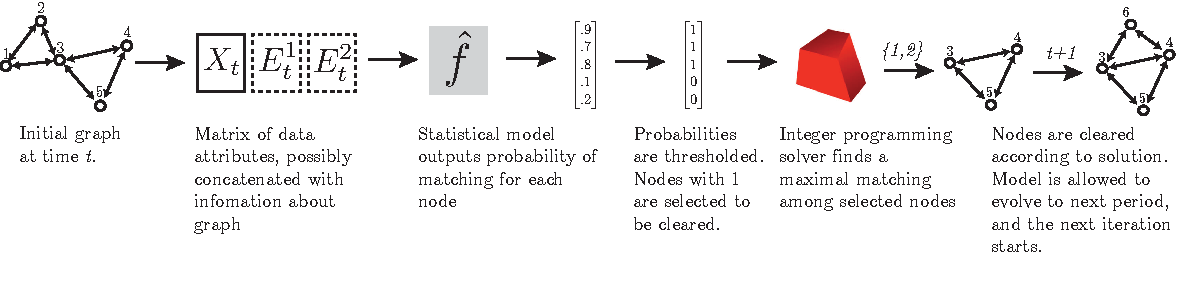
\includegraphics[width=\textwidth]{/Users/vitorhadad/Documents/kidney/matching/phd_thesis/figures/direct_prediction.pdf}.
\caption{One period of simulation using direct prediction methods to choose cycles.}
\label{fig:direct_prediction}
\end{figure}


\section{Results}

\subsection{Direct estimation policy}

In order to produce data to feed into our ``classifier", we simulated and solved a 1000-period run environment was simulated and solved using OPT using with each each node's observable characteristics as regressors, and a binary variable indicating whether they were matched or not as the regressand. The resulting artificial dataset of approximately 2 million observations was then fed to a series of predictive algorithms, including penalized logistic regression\citep{wu2009genome}, support vector machines with radial basis function kernels\citep{cortes1995support}, random forest classifiers\citep{breiman2001random}, gradient tree boosting classifiers\citep{friedman2001greedy} and deep feedforward networks\citep{goodfellow2016deep}. The performance of these algorithms as classification methods is compared in Table \ref{tab:direct_prediction} in the Supplementary Material section.

\subsection{MAB-based policy}

We have access to the data-generating process (\emph{environments}) and an algorithm that is able to find the best matching for any data in hindsight (\texttt{OPT}). Therefore, in principle we could estimate the best choice of cycle to clear by simulating several periods ahead in the future, running \texttt{OPT}, and measuring the performance of our choice under any desired criterion. 

The approach outlined above turns out to be naive and incomplete, but it essentially contains the insight under which we will be working in this section. It is naive because simulations are computationally expensive, and in practice we cannot repeat them enough times get reliable estimates of the average performance for each cycle choice, especially in large graphs. It is also incomplete because it does not specify exactly what is the best information we should extract from \texttt{OPT} results. In order to solve the first problem, we leverage theory and algorithms from the multi-armed bandit (MAB) literature. For the second, we propose a secondary objective based on what we call \emph{pseudo-rewards}.

Our procedure is illustrated in Figures \ref{fig:mab} and \ref{fig:mab_step}. At the beginning of the period $t$, the agent receives a set of cycles $C$ that are available to be cleared. If $C$ is empty, nothing happens and we move to the next period. Otherwise, the agent then picks a cycle $c \in C$ and simulates the future, including new entries and deaths, up to a horizon $h$. Next, \texttt{OPT} is run twice, once normally, and once with the additional constraint that $c$ be removed today. The size of the resulting matching in these two scenarios is compared. Naturally, the constrained version of \texttt{OPT} cannot achieve anything better than its unconstrained counterpart, but it might get to be equal. If it is, the agent receives a \emph{pseudo-reward} of one, otherwise it receives zero. This process is repeated: at each iteration $\ell$, a cycle $c_{\ell}$ is chosen and its pseudo-reward $r_{c, \ell}$ is revealed. When a preset computational budget of $L(|C|)$ iterations is hit, the agent then analyses the whole history of cycle choices and pseudo-rewards $H_{t} = \{ (c_{\ell}, r_{c\ell} ) \}_{\ell=1}^{L}$, and decides whether to match one of the cycles or move on to the next period. If a cycle $c$ is chosen it is immediately cleared, however the environment does not evolve to the next period yet. Instead, the history $H_t$ is discarded the procedure is repeated again with a reduced set of actions $C' \subset C$ that produces a new history $H_t'$ and so on, until either there are no more available choices or the agent decides to allow the environment to move on to time $t+1$. When that at last happens, entries and deaths are revealed, the agent receives a new set of cycles, and the process begin anew. All past information is ignored.


Two important details were left out of the explanation above. First, how does the agent chooses the next cycle to test? Second, how does it decide which cycle to choose (or no cycle at all)? 

Let $c^{*}$ be a cycle that maximizes expected pseudo-rewards during one round of the algorithm:
$$c_{\ell}^{*} \in \arg\max_{c} E[r_{c,\ell}] $$


 Also, let \emph{regret} be defined as the difference between expected reward of the optimal choice $c^*$ and its own selected choice $c_{\ell}$.
 
 $$\Delta_\ell := E[r_{c^{*},\ell}] - E[r_{c,\ell}]$$
 
 A \emph{multi-armed bandit} (MAB) algorithm is a procedure to minimize the cumulative regret over $L$ rounds. A good MAB algorithm will act so as to balance exploration (trying out different choices to get high-quality estimates of their rewards) and exploitation (using out better choices more often to increase total rewards). 
 
 The literature on bandit algorithms is extensive and spans at least seventy years of research \citep{lattimore2018bandits}. Here we will focus on binary 
 
 
 

 \begin{figure}
  \centering
  %\hspace{-1cm}
  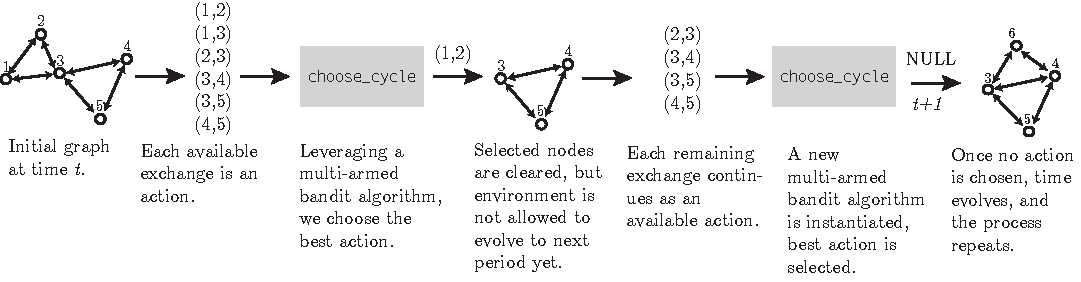
\includegraphics[width=1\textwidth]{/Users/vitorhadad/Documents/kidney/matching/phd_thesis/figures/mab.pdf}
  \caption{One period of simulation using multi-armed bandit methods to choose cycles.}
  \label{fig:mab}
  \end{figure}

  \begin{figure}
  \centering
  %\hspace*{-0.5cm}
  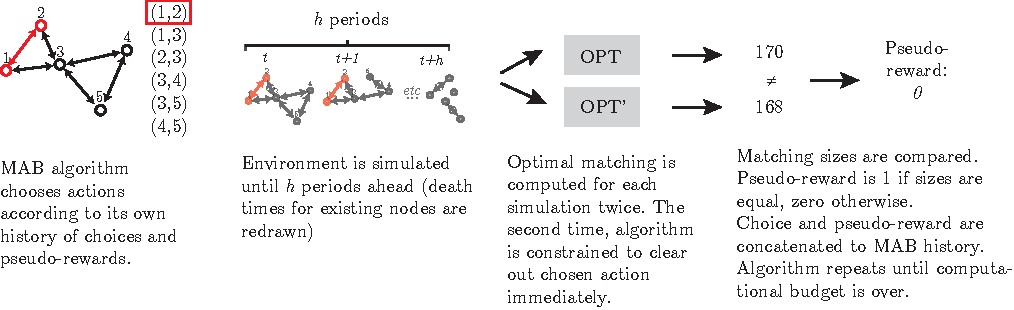
\includegraphics[width=1\textwidth]{/Users/vitorhadad/Documents/kidney/matching/phd_thesis/figures/mab_step.pdf}
  \caption{\textbf{Function} \textsc{get\_pseudo\_reward} \\ Multi-armed bandits evaluate if a cycle should be cleared by checking if there is a high chance that the cycle will be used in the future. Such cycles get a \emph{lower} reward, and are left for later.}
  \label{fig:get_pseudo_reward}
  \end{figure}




  
\paragraph{What are pseudo-rewards?} Figure \ref{fig:pseudo_reward_intuition}


\begin{figure}[htbp]
\centering
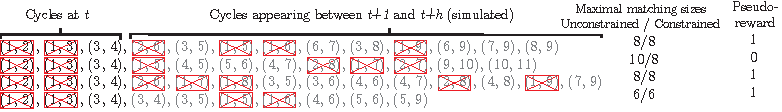
\includegraphics[width=0.95\textwidth]{/Users/vitorhadad/Documents/kidney/matching/phd_thesis/figures/pseudo_reward_intuition.pdf}
\caption{Pseudo-reward intuition}
\label{fig:pseudo_reward_intuition}
\end{figure}


\section{Conclusion}

\paragraph{Summary}

\paragraph{Extensions} In reality, some exchanges are more or less desirable than others, either for ethical concerns or because of predicted health benefit. For example, it is common for pediatric patients and previous organ donors receive higher priority, as do exchanges involving patients with no HLA mismatch. 


% Algorithm
\begin{algorithm}[htbp]
	\SetAlgoLined
	\KwData{Cycle $c$; Horizon $h$; \\
          Lists pseudo-reward statistics $Avg$, $Std$; \\
          Environment simulator object \textsc{Env}; \\
          Oracle solver \textsc{OPT}; }
  \DontPrintSemicolon
  \SetKwFunction{FChoose}{\textsc{get\_pseudo\_reward}}
  \SetKwProg{Fn}{Function}{:}{}
  \Fn{\FChoose{\textsc{Env}, \ $c$, \ $Avg$, \ $Std$, \ $h$ }}{
    \tcp{Simulate up to horizon $h$ and find optimal matching} \\
    \textsc{Env.simulate}($h$)  \\
    $r_1$ \gets \textsc{OPT.solve}(\textsc{Env})  \\
    \tcp{Remove cycle $c$, find constrained optimal matching} \\
    \textsc{Env.remove}($c$)  \\
    $r_2$ \gets \textsc{OPT.solve}(\textsc{Env}) \\
    \tcp{Return 1 if rewards are equal, 0 otherwise} \\
    \KwRet $r_1 == r_2$ \;
  }
	\caption{Function \textsc{get\_pseudo\_reward}}
	\label{alg:get_pseudo_reward}
\end{algorithm}



\begin{algorithm}[htbp]
	
  \SetAlgoLined
  \DontPrintSemicolon
	
  \KwData{Horizon $h$; Number of iterations $L$; Threshold $thres$; \\
    Environment simulator object \textsc{Env};
    Multi-armed bandit algorithm object \textsc{MAB};
  }

  \SetKwFunction{FChoose}{\texttt{choose\_cycle}}
  \SetKwProg{Fn}{Function}{:}{}
  
  \Fn{\FChoose{\texttt{Env},\ \texttt{h} }}{
    \tcp{Initialize lists of current pseudo-reward statistics} \\
    $C$ \gets \textsc{Env.get\_available\_cycles()} \\
    $Avg$ \gets \textsc{zeros(length(C))} \\
    $Std$ \gets \textsc{zeros(length(C))} \\
    
    \tcp{Begin iterations} \\
    \For{$i\gets0$ \KwTo $L$}{
      \tcp{Bandit algorithm chooses next cycle to test given statistics} \\
      $c$ \gets \textsc{MAB.pull($C$, Avg, Std)}  \\
      \tcp{Compute pseudo reward for this cycle and update statistics} \\
      $r$ \gets \textsc{get\_pseudo\_reward}(\textsc{Env},\ $c$,\ $Avg$,\ $Std$,\ $h$) \\
      $Avg$ \gets \textsc{update\_running\_average($Avg$, $r$)} \\
      $Std$ \gets \textsc{update\_running\_std($Std$, $r$)} \\ 
    }  
    \tcp{Bandit algorithm chooses best cycle given statistics} \\
    $c\_best$ \gets \textsc{MAB.choose($C$, Avg, Std)} \\
    \tcp{Return best cycle, unless none of the pseudo-reward averages are above a certain threshold} \\
    \eIf{\textsc{All}($Avg \leq thres$)} {
      \KwRet \text{NULL} \\ 
      }{
      \KwRet $c$ \\
      }
    }
  }
	\caption{Function \texttt{choose\_cycle}}
	\label{alg:choose_cycle}
\end{algorithm}




\section{Conclusions}



% Appendix
\appendix
\section{Sections}

\section{Supplementary materials}

\begin{acks}
	
% The author would like to thank Utku \"{U}nver, Stefan Hoderlein, Arthur Lewbel, Mohammad Akbarpour, Itai Ashlagi, David Parkes, John Dickerson, Enkhmanlai Amarsaikhan and Sainbayar Sukhbaatar for helpful discussions.

The author would like to thank Itai Ashlagi for the idea of including a donor cPRA in the OPTN environment.

This work was supported in part by Health Resources and Services Administration contract 234-2005-37011C. The content is the responsibility of the authors alone and does not necessarily reflect the views or policies of the Department of Health and Human Services, nor does mention of trade names, commercial products, or organizations imply endorsement by the U.S. Government.

	
\end{acks}

% Bibliography
\bibliographystyle{ACM-Reference-Format}
\bibliography{/Users/vitorhadad/Documents/kidney/matching/phd_thesis/references}

\end{document}
